\documentclass[a4paper,12pt,twoside]{article}
\usepackage[utf8]{inputenc}
\usepackage[T1]{fontenc}
\usepackage{graphicx}
\usepackage{anysize}
\usepackage{enumerate}
\usepackage{amssymb}
\usepackage[polish]{babel}

%\marginsize{left}{right}{top}{bottom}
\marginsize{2.5cm}{2.5cm}{2.5cm}{2.5cm}
\sloppy

\begin{document}



\section{Środowisko \emph{minipage}}

Nauka zajmująca się badaniem i poznawaniem budowy organizmów ptaków oraz ich życia nosi nazwę ornitologii i jest częścią zoologii. Do tej dyscypliny naukowej należy morfologia, tj. nauka o wyglądzie i budowie zewnętrznej i wewnętrznej ptaka, biologia - nauka o wszelkich przejawach ich życia fizycznego: ekologia, nauka o wymaganych przez dany gatunek warunkach środowiskowych oraz etologia - nauka o zwyczajach i sposobie zachowania się poszczególnych gatunków. W zakres wiedzy ornitologicznej wchodzi również systematyka zoologiczna, polegająca na podziale wszystkich ptaków na grupy systematyczne (gromada, rząd, rodzina, rodzaj, gatunek) według bliższego lub dalszego pokrewieństwa.\footnotetext{Przypis w tekście głównym.}

\medskip

\begin{minipage}{8cm}
Niezależnie od systematyki przyjęto tutaj podział wszystkich ptaków na trzy grupy według ich użyteczności gospodarczej:
\begin{enumerate}[i)]
\item ptaki łowne, które w okresie lęgów znajdują się pod tzw. ochroną okresową,
\item ptaki objęte całoroczną ochroną, zwaną gatunkową,
\item ptaki, które w ciągu całego roku w ogóle nie podlegają ochronie.\footnotetext{Przypis w środowisku minipage.}
\end{enumerate}
\end{minipage}

\vspace{1cm}

\begin{minipage}{8cm}
Niezależnie od systematyki przyjęto tutaj podział wszystkich ptaków na trzy grupy według ich użyteczności gospodarczej:
\begin{enumerate}[i)]
\item ptaki łowne, które w okresie lęgów znajdują się pod tzw. ochroną okresową,
\item ptaki objęte całoroczną ochroną, zwaną gatunkową,
\item ptaki, które w ciągu całego roku w ogóle nie podlegają ochronie.
\end{enumerate}
\end{minipage}
%
\hspace{5mm}
%
\begin{minipage}{7cm}
\centerline{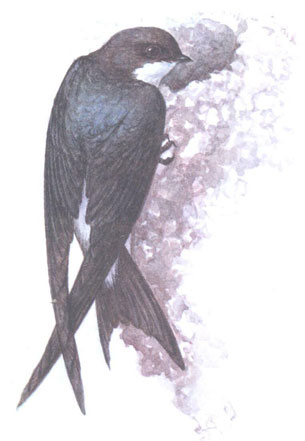
\includegraphics[scale=0.35]{jaskolka-oknowka}}
\end{minipage}

\newpage


\paragraph{Gawron} Pospolity gatunek osiadły i zalatujący. Przebywa najchętniej na terenach nizinnych w zagajnikach, alejach, parkach. Na terenach pagórkowatych występuje rzadko. W zimie stada gawronów pojawiają się w wielkich ilościach na polach oraz w osiedlach ludzkich, przeważnie są to osobniki z krajów położonych na północny wschód od Polski. Gnieździ się w koloniach na skrajach lasów, w zagajnikach i dużych parkach. Gniazdo umiejscawia na wysokich drzewach z dobrze rozwiniętą koroną. Jest ono dość niestarannie zbudowane z suchych gałązek trawy i suchych korzonków, wewnątrz wysłane sierścią.

\medskip

\begin{minipage}[t][6cm][t]{45mm}
Gatunek monogamiczny. Okres gniazdowania: marzec - kwiecień. Samica znosi 3 - 5 jaj. Jaja wysiaduje samica przez 18 - 19 dni. Pisklęta są gniazdownikami. Rodzice karmią młode przez 28-30 dni.  
\end{minipage}
%
\hspace{5mm}
%
\begin{minipage}[t][6cm][c]{45mm}
Gatunek monogamiczny. Okres gniazdowania: marzec - kwiecień. Samica znosi 3 - 5 jaj. Jaja wysiaduje samica przez 18 - 19 dni. Pisklęta są gniazdownikami. Rodzice karmią młode przez 28-30 dni. 
\end{minipage}
%
\hspace{5mm}
%
\begin{minipage}[t][6cm][b]{45mm}
Gatunek monogamiczny. Okres gniazdowania: marzec - kwiecień. Samica znosi 3 - 5 jaj. Jaja wysiaduje samica przez 18 - 19 dni. Pisklęta są gniazdownikami. Rodzice karmią młode przez 28-30 dni.  
\end{minipage}

\newpage

\paragraph{Gawron} Pospolity gatunek osiadły i zalatujący. Przebywa najchętniej na terenach nizinnych w zagajnikach, alejach, parkach. Na terenach pagórkowatych występuje rzadko. W zimie stada gawronów pojawiają się w wielkich ilościach na polach oraz w osiedlach ludzkich, przeważnie są to osobniki z krajów położonych na północny wschód od Polski. Gnieździ się w koloniach na skrajach lasów, w zagajnikach i dużych parkach. Gniazdo umiejscawia na wysokich drzewach z dobrze rozwiniętą koroną. Jest ono dość niestarannie zbudowane z suchych gałązek trawy i suchych korzonków, wewnątrz wysłane sierścią.

\medskip

\begin{minipage}[t][7cm][c]{45mm}
Gatunek monogamiczny. Okres gniazdowania: marzec - kwiecień. Samica znosi 3 - 5 jaj. Jaja wysiaduje samica przez 18 - 19 dni. Pisklęta są gniazdownikami. Rodzice karmią młode przez 28-30 dni.  
\end{minipage}
%
\hspace{5mm}
%
\begin{minipage}[c][7cm][c]{45mm}
Gatunek monogamiczny. Okres gniazdowania: marzec - kwiecień. Samica znosi 3 - 5 jaj. Jaja wysiaduje samica przez 18 - 19 dni. Pisklęta są gniazdownikami. Rodzice karmią młode przez 28-30 dni. 
\end{minipage}
%
\hspace{5mm}
%
\begin{minipage}[b][7cm][c]{45mm}
Gatunek monogamiczny. Okres gniazdowania: marzec - kwiecień. Samica znosi 3 - 5 jaj. Jaja wysiaduje samica przez 18 - 19 dni. Pisklęta są gniazdownikami. Rodzice karmią młode przez 28-30 dni.  
\end{minipage}

\newpage


\hfill
\begin{minipage}[t][\textheight][b]{45mm}
Gatunek monogamiczny. Okres gniazdowania: marzec - kwiecień. Samica znosi 3 - 5 jaj. Jaja wysiaduje samica przez 18 - 19 dni. Pisklęta są gniazdownikami. Rodzice karmią młode przez 28-30 dni.  
\end{minipage}

\end{document}

